\chapter{Układ sterowania i instrumentacji}
\label{cha:ch3_uklad_ster_i_instrumentacji}

Do odczytywania danych z obiektu i sterowania nim wykorzystano opisany w tym rozdziale układ sterowania i instrumentacji (\cref{fig:schemat_ukl_sterowania_instrumentacji}). W jego sercu znajduje się przemysłowy sterownik PLC, który odczytuje dane o położeniu kulki z dwóch czujników odległości oraz położenie kątowe wału silnika z~enkodera. Dodatkowo do sterownika podłączony został czujnik bazowania oraz przyciski: \texttt{START} (NO), \texttt{STOP} (NC). Na wyjścia sterownika podłączony został mostek H kontrolujący silnik oraz dioda sygnalizacyjna.

% TODO: zweryfikować podłączenie przycisków

\begin{figure}[H]
    \centering
    % TODO: przerobić rysunek w Inkscape
    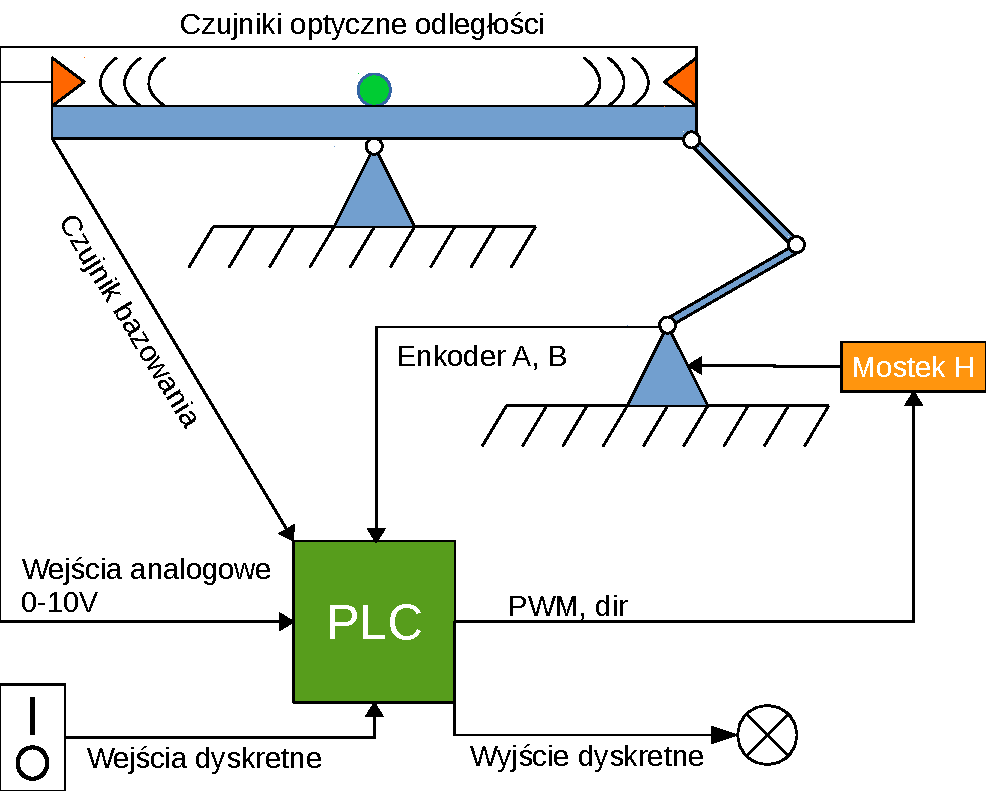
\includegraphics[width=0.7\textwidth]{schemat_ukladu3}
    \caption{Schemat układu sterowania i instrumentacji wraz z zaznaczonymi połączeniami.}
    \label{fig:schemat_ukl_sterowania_instrumentacji}
\end{figure}

%%%%%%%%
\section{Sterownik PLC}
\label{sec:ch3_PLC}

Wykorzystany w pracy sterownik PLC to Siemens S7-1211C DC/DC/DC. Działa on na napięciu stałym \SI{24}{V}, posiada 6 wejść dyskretnych \SI{24}{V}, 4 tranzystorowe wyjścia dyskretne \SI{24}{V} i 2 napięciowe wejścia analogowe \SIrange{0}{10}{V}.

W celu ułatwienia komunikacji między sterownikiem i elektroniką opartą o logikę \SI{5}{V} (więcej w podrozdziale \ref{sec:ch3_systemy_napiec}), został on rozszerzony o dodatkową płytkę sygnałową SB 1223 działającą na logice \SI{5}{V}; dodaje ona po 2 wejścia i~wyjścia dyskretne \SI{5}{V}.

Podstawowe parametry sterownika oraz płytki sygnałowej zostały zebrane w tabeli \ref{tab:parametry_PLC_SB}:

\begin{table}[H]
    \centering
    \begin{threeparttable}
        \caption{Podstawowe parametry sterownika PLC Siemens S7-1211C i płytki sygnałowej Siemens SB 1223\tnote{a}.}
        \label{tab:parametry_PLC_SB}
        
        \begin{tabularx}{\textwidth}{p{5cm} | p{5cm} | p{5cm} }
            \toprule
            Nazwa & Siemens S7-1211C & Siemens SB 1223 \\
            \midrule
            Napięcie zasilania & \SI{24}{V} DC & \SI{5}{V} DC \\
            \midrule
            Ilość wejść cyfrowych & 6 & 2 \\
            Ilość wyjść cyfrowych & 4 & 2 \\
            Ilość wejść analogowych & 2 & 0 \\
            Ilość wyjść analogowych & 0 & 0 \\
            Typ wejść cyfrowych & \textit{sink-source} & \textit{source} \\
            Typ wyjść cyfrowych & półprzewodnikowe MOSFET \textit{source} & półprzewodnikowe MOSFET \textit{sink-source} \\
            Typ wejść analogowych & Napięciowe \SIrange{0}{10}{V} & n.d. \\
            \midrule
            Szybkie liczniki & Do 6 z częstotliwością \SI{100}{kHz}\tnote{b} & Do 2 z częstotliwością \SI{200}{kHz}\tnote{c} \\
            Wyjścia impulsowe & Do 4 z częstotliwością \SI{100}{kHz} & Do 2 z częstotliwością \SI{200}{kHz} \\
            \midrule
            Pamięć robocza & \SI{30}{kB} & n.d. \\
            Pamięć ładowania & \SI{1}{MB} & n.d. \\
            Pamięć trwała & \SI{10}{kB} & n.d. \\
            \midrule
            Czas wykonywania instrukcji boolowskich & \SI{0,08}{\micro\second}/instrukcję & n.d. \\
            Czas wykonywania operacji na typie WORD & \SI{1,7}{\micro\second}/instrukcję & n.d. \\
            Czas wykonywania operacji na typie REAL & \SI{2,3}{\micro\second}/instrukcję & n.d. \\
            \bottomrule
        \end{tabularx}
        
        \begin{tablenotes}
            \footnotesize
            \item[a] opracowanie własne na podstawie \cite{S7MANUAL},
            \item[b] w trybie kwadraturowym wykorzystywane są dwa wejścia, a~maksymalna częstotliwość wynosi \SI{80}{kHz},
            \item[c] w trybie kwadraturowym wykorzystywane są dwa wejścia, a~maksymalna częstotliwość wynosi \SI{160}{kHz}.
        \end{tablenotes}
    \end{threeparttable}
\end{table}

% TODO: dodaj zdjęcia

%%%%%%%%
\section{Silnik z reduktorem i enkoderem}
\label{sec:ch3_uklad_napedowy}

Jak już zasygnalizowano w rozdziale \ref{sec:ch2_przeniesienie_napedu}, w pracy użyto silnika prądu stałego (komutatorowy, z~magnesami trwałymi). Silnik sprzężony jest z~zębatą przekładnią redukcyjną o przełożeniu \num{18,75}:\num{1}. Za silnikiem umieszczony jest enkoder inkrementalny kwadraturowy o~64 impulsach na obrót wału, co daje 1200 impulsów za przekładnią.

Wybrany silnik stanowi dobry kompromis między złożonością, wydajnością i ceną. Dyskusja na temat możliwości zastosowania innych typów napędów została przeprowadzona w dodatku \ref{appA_warianty_zespolu_napedowego}.

Producent silnika nie dostarcza pełnej dokumentacji, a jedynie kilka wybranych parametrów. Wymusiło to analityczne lub eksperymentalne wyznaczenie pozostałych wymaganych do zamodelowania silnika parametrów. Wszystkie parametry zostały przedstawione w tabeli \ref{tab:parametry_silnika} poniżej.

\begin{table}[h]
    \centering
    \begin{threeparttable}
        \caption{Parametry producenta silnika, enkodera i przekładni\tnote{a}.}
        \label{tab:parametry_silnika}
        
        \begin{tabularx}{0.9\textwidth}{l | l}
            \toprule
            Parametr & Wartość \\
            \midrule
            Średnica & \SI{37}{\milli\meter} \\
            Długość & \SI{68}{\milli\meter} \\
            Masa & \SI{215}{g} \\
            Średnica wału & \SI{6}{\milli\meter} \\
            \midrule
            Przełożenie przekładni & \num{18,75}:\num{1} \\
            \midrule
            Napięcie znamionowe & \SI{12}{\volt} \\
            Prędkość znamionowa & \SI{52,36}{\radian\per\second} \\
            Prąd znamionowy & \SI{300}{\milli\ampere} \\
            Prąd zatrzymania silnika & \SI{5000}{\milli\ampere} \\
            Moment zatrzymania silnika & \SI{0,59}{\newton\meter} \\
            \midrule
            Typ enkodera & Kwadraturowy, inkrementalny, bez pamięci \\
            Ilość impulsów na obrót za przekładnią & \num{1200} (tryb kwadraturowy) \\
%            Rezystancja\tnote{b} & \SI{2,4}{\ohm} \\
%            Stała SEM rotacji\tnote{b} $K_e$ & \SI{0,2154}{\volt\per\radian\per\second} \\
%            Stała momentu\tnote{b} $K_t$ & \SI{0,2154}{\newton\meter\per\ampere} \\
%            Współczynnik tarcia wiskotycznego\tnote{b} $\beta$ & \num{0,00161} \\
%            Współczynnik tarcia suchego\tnote{b} $b$ & \num{0,019} \\
%            Moment bezwładności przekładni i wału\tnote{c} $J$ & \num{0,00123} \\
            \bottomrule
        \end{tabularx}
        
        \begin{tablenotes}
            \footnotesize
            \item[a] opracowanie własne na podstawie \cite{SILNIK_MANUAL}.
%            \item[b] zidentyfikowano analitycznie, więcej w rozdziale \ref{cha:ch6_identyfikacja},
%            \item[b] zidentyfikowano eksperymentalnie, więcej w rozdziale \ref{cha:ch6_identyfikacja}.
        \end{tablenotes}
    \end{threeparttable}
\end{table}

Parametry niewymienione w tabeli \ref{tab:parametry_silnika}, takie jak rezystancja silnika, stała silnika, moment bezwładności wału czy współczynniki tarcia suchego i wiskotycznego, nie zostały podane przez producenta, dlatego została przeprowadzona ich identyfikacja opisana w rozdziale \ref{cha:ch6_identyfikacja}.

Silnik sterowany jest przez PLC za pomocą układu mostka H (Pololu BD65496MUV). Został on dobrany tak, by spełniać wymagania elektryczne silnika w pracy znamionowej. Sterowany jest sygnałem PWM o częstotliwości przenoszenia \SI{20}{\kilo\hertz}. Dodatkowym sygnałem jest binarny sygnał kierunku obrotu silnika. Najistotniejsze parametry wybranego mostka H przedstawiono w tabeli \ref{tab:parametry_mostka_H}.

\begin{table}[h]
    \centering
    \begin{threeparttable}
        \caption{Najważniejsze parametry mostka H\tnote{a}.}
        \label{tab:parametry_mostka_H}
        
        \begin{tabularx}{0.7\textwidth}{l | l}
            \toprule
            Parametr & Wartość \\
            \midrule
            Napięcie pracy silnika & \SIrange{2}{16}{\volt} \\
            Maksymalny prąd ciągły silnika & \SI{1,2}{\ampere} \\
            Maksymalny prąd chwilowy silnika & \SI{5}{\ampere} \\
            Maksymalna częstotliwość PWM & \SI{500}{\kilo\hertz} \\
            Napięcie zasilania & \SIrange{2,5}{5,5}{\volt} \\
            Napięcie sygnałów logicznych & Napięcie zasilania \SI{+-0,3}{\volt} \\
            \bottomrule
        \end{tabularx}
        
        \begin{tablenotes}
            \footnotesize
            \item[a] opracowanie własne na podstawie \cite{MOSTEK_H_MANUAL}.
        \end{tablenotes}
    \end{threeparttable}
\end{table}

Mostek H przylutowano do płytki uniwersalnej. Połączenia elektryczne zrealizowano za pomocą przylutowanych czterech podwójnych złączy ARK (raster \SI{2,54}{\milli\meter}). Zdjęcie modułu przedstawiono na figurze \ref{fig:zdjecie_mostka_H}, a opis złącz w tabeli \ref{tab:zlacza_mostka_H}.

\begin{figure}[H]
    \centering
    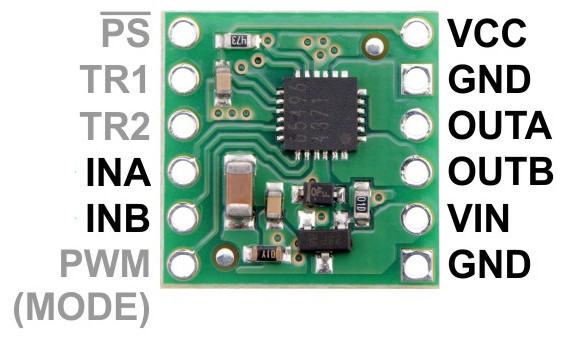
\includegraphics[width=0.4\textwidth]{mostek_H}
    \caption{Zdjęcie układu mostka H (Pololu BD65496MUV). Źródło: \url{https://www.pololu.com/product/2960}.}
    \label{fig:zdjecie_mostka_H}
\end{figure}

\begin{table}[h]
    \centering
    \begin{threeparttable}
        \caption{Opis złącz mostka H\tnote{a}.}
        \label{tab:zlacza_mostka_H}
        
        \begin{tabularx}{0.67\textwidth}{l | l}
            \toprule
            Złącze & Opis \\
            \midrule
            \texttt{VCC} & Zasilanie układu \\
            \texttt{VIN} & Zasilanie silnika \\
            \texttt{GND} & Masa \\
            \texttt{OUTA}, \texttt{OUTB} & Wyjścia zasilania silnika \\
            \texttt{INA}, \texttt{INB} & Wejścia sygnałów sterujących \\
            \texttt{PWM (MODE)} & Przełączanie między trybem \texttt{IN/IN} a~\texttt{EN/IN}\tnote{b} \\
            \texttt{PS} & Oszczędzanie energii \\
            \texttt{TR1}, \texttt{TR2} & Kontrola maksymalnej częstotliwości \\
            \bottomrule
        \end{tabularx}
        
        \begin{tablenotes}
            \footnotesize
            \item[a] opracowanie własne na podstawie \cite{MOSTEK_H_MANUAL},
            \item[b] układ umożliwia sterowanie silnikiem w trybie \texttt{IN/IN} oraz \texttt{EN/IN}; ten pierwszy przekazuje sygnał wysoki ze złącza \texttt{INA} na \texttt{OUTA} i \texttt{INB} na \texttt{OUTB} (za wyjątkiem sytuacji dwóch stanów wysokich), natomiast ten drugi pozwala użyć sygnału PWM (\texttt{INA}) oraz sygnału kierunku obrotu (\texttt{INB}).
        \end{tablenotes}
    \end{threeparttable}
\end{table}

%%%%%%%%
\section{Czujniki odległości}
\label{sec:ch3_czujniki_odleglosci}

Do pomiaru położenia kulki wykorzystano parę analogowych czujników Sharp GP2Y0A41SK0F. Każdy z czujników składa się z nadajnika światła podczerwonego i odbiornika; obliczanie pozycji obiektu odbywa się na zasadzie triangulacji. Podstawowe parametry czujników opisano w tabeli \ref{tab:parametry_czujnikow_Sharp}.

Czujniki optyczne pracujące w podczerwieni nie są jedynymi sensorami, które można zastosować do badania położenia kulki w układach typu kulka i belka. Alternatywne sposoby zostały omówione w~dodatku \ref{appB_alternatywne_czujniki_pozycji_kulki}.

\begin{table}[h]
    \centering
    \begin{threeparttable}
        \caption{Podstawowe parametry czujników pozycji kulki\tnote{a}.}
        \label{tab:parametry_czujnikow_Sharp}
        
        \begin{tabularx}{0.55\textwidth}{l | l}
            \toprule
            Parametr & Wartość \\
            \midrule
            Napięcie zasilania & \SIrange{4,5}{5,5}{\volt} \\
            Zasięg & \SIrange{4}{30}{\centi\meter} \\
            Typ sygnału & Analogowy około \SIrange{0,25}{3,1}{\volt} \\
            \bottomrule
        \end{tabularx}
        
        \begin{tablenotes}
            \footnotesize
            % TODO: dodaj manual SHARP do bibliografii
            \item[a] opracowanie własne na podstawie \cite{SHARP_MANUAL}.
        \end{tablenotes}
    \end{threeparttable}
\end{table}

Czujniki zostały zamontowane na uchwytach umożliwiających regulację wysokości oraz pochylenia względem belki (zob. rozdział \ref{sec:ch2_belka}). Odległość między czujnikami to \SI{40}{\centi\meter} (powyżej górnej granicy zakresu pracy), a ich wysokość nad belką to \SI{4}{\centi\meter}.

Charakterystyka każdego z czujników jest mocno nieliniowa (zob. \cref{fig:charakterystyka_czujnikow}). Dobrą aproksymację charakterystyki można otrzymać (po odcięciu wartości poniżej \SI{3}{\centi\meter}) za pomocą funkcji postaci $y = a x ^ b + c$ (zob. tabela \ref{tab:aproksymacja_czujnikow})\footnote{Wzór właściwy dla odległości do kulki w funkcji wartości z czujnika, tj. po ,,zamianie'' osi wykresu z figury \ref{fig:charakterystyka_czujnikow}.}, jednakże z powodu dużej złożoności obliczeniowej liczenia potęg niecałkowitych zrezygnowano z implementacji takich aproksymacji w sterowniku PLC.

\begin{figure}[h]
    \centering
    % \includesvg[width=0.8\textwidth,svgpath=./graphics/]{sensor_characteristics}
    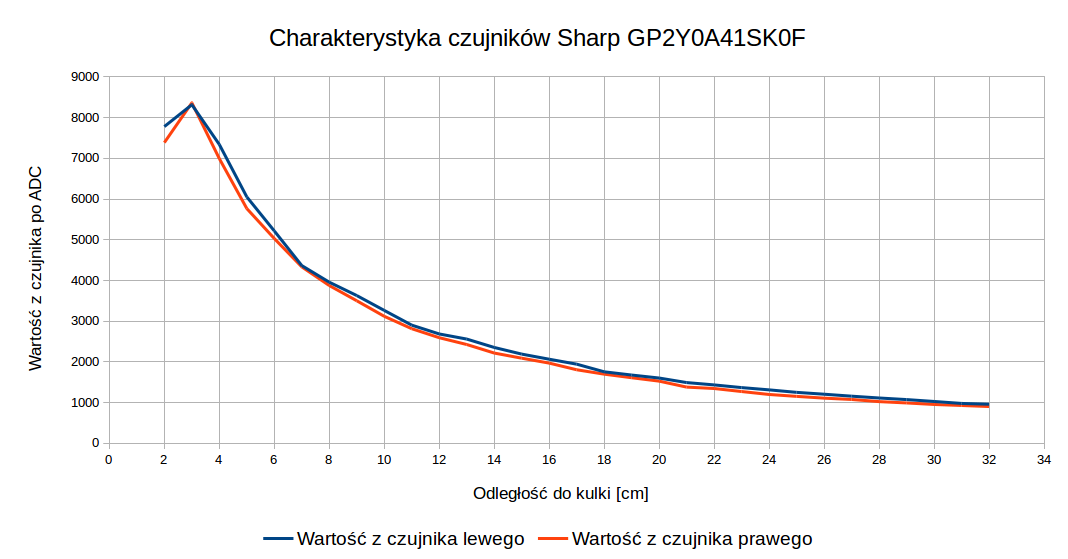
\includegraphics[width=1\textwidth]{sensor_characteristics}
    \caption{Charakterystyka czujników odległości.}
    \label{fig:charakterystyka_czujnikow}
\end{figure}

\begin{table}[h]
    \centering
    \begin{threeparttable}
        \caption{Funkcje aproksymujące charakterystyki czujników.}
        \label{tab:aproksymacja_czujnikow}
        
        \begin{tabularx}{0.4\textwidth}{l | l}
            \toprule
            Czujnik & Funkcja aproksymująca \\
            \midrule
            Lewy\tnote{a}  & $y = 9819 x ^ {-0.8229} - 2.651 $ \\
            Prawy\tnote{a} & $y = 8166 x ^ {-0.8055} - 2.525 $ \\
            \bottomrule
        \end{tabularx}
        
        \begin{tablenotes}
            \footnotesize
            \item[a] czujnik określony jako ,,lewy'' jest bardziej oddalony od zespołu napędowego.
        \end{tablenotes}
    \end{threeparttable}
\end{table}

Wobec utrudnień spowodowanych złożonością obliczeniową zastosowano inne rozwiązanie w celu obliczenia pozycji kulki: aproksymację liniową pomiędzy punktami charakterystyki. W tym celu wprowadzono punkty charakterystyki każdego z czujników (pary: wartość z czujnika po przetworniku ADC, odległość do kulki) do dwóch tablic w sterowniku PLC.

% TODO: opisz sposób liczenia położenia kulki

%%%%%%%%
\section{Czujnik bazowania}
\label{sec:ch3_czujnik_bazowania}

% TODO: transoptor szczelinowy, sposób montażu, schemat połączeń

%%%%%%%%
\section{Okablowanie i zabezpieczenia}
\label{sec:ch3_okablowanie_zabezpieczenia}

% TODO: zdjęcie "szafy"

%%%%%%%%
\section{Systemy napięć}
\label{sec:ch3_systemy_napiec}

% TODO: 5V, 12V, 24V

%%%%%%%%
\section{Podsumowanie}


%---------------------------------------------------------------------------